{\textbf{1. 树的基本概念}}

树是n(n≥0)个结点的有限集合T。当n=0时,称为空树;当n\textgreater{}0时,该集合满足如下条件:

{1.
其中{必有一个称为根的特定结点},它没有直接前驱,但有零个或多个直接后继(如结点a)。}

{2. 其余n-1个结点可以划分为m(m≥0)个互不相交的有限集合T1,T2,
,Tm,其中Ti又是一棵树,称为根root的子树。每棵子树的根结点有且仅有一个直接前驱,但有零个或多个直接后继。}

{\textbf{2. 树相关术语}}

{\textbf{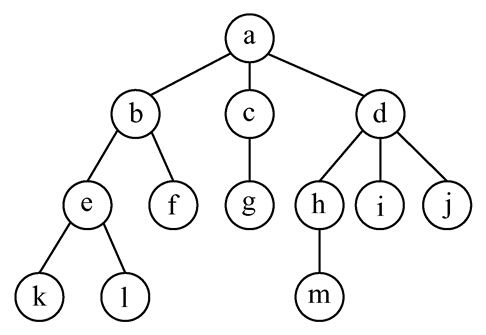
\includegraphics[width=2.08333in,height=2.08333in]{png-jpeg-pics/a16db4da9e6fde364685db7c67e3b509?}\\
}}

{1. 结点:a、b、
m都是结点,结点不仅包含数值元素,而且包含指向子树的分支。如结点a包含指向b、c、d这3个子树的指针。}

{2. 结点的度:结点拥有的子树个数(即分支个数)。如结点A的度为3。}

{3. 叶子结点(终端结点):指度为0的结点,如f、g、i、j、k、l、m。}

{4. 非终端结点:指度不为0的结点,如a、b、c、d、e、h。}

{5. 孩子:结点的子树的根,如a结点的孩子包括b、c、d这3个结点。}

{6. 双亲(父结点):如b、c、d的双亲都是a。}

{7. 兄弟:如b、c、d互为兄弟。}

{8.
祖先:从根到某结点的路径上的所有结点,都是这个结点的祖先。如k的祖先是a、b、e。}

{9.
子孙(子树结点):从某结点为根的子树中的所有结点,都是该结点的子孙。如d的子孙为h、i、j、m。}

{10. 层次:从根开始,根为第一层,根的孩子们为第二层,以此类推。}

{11.
树的高度(或深度):树中结点的最大层次。如例子中高度(或深度)为4。}

{12.
结点的深度和高度:结点深度是从根结点算起的,而结点高度是从最底层的}{叶子结点算其的。如结点g的高度为2,深度为3。}

{13.
堂兄弟:双亲在同一层(但不是同一个)的结点互为堂兄弟。如f、g、h都互为堂兄弟。}

{14.
有序树:树中结点的子树从左到右是有次序的,不能交换的,这样的树称为有序树。}

{15. 无序树:就是子树无次序,可任意交换的树称为无序树。}

{16.
森林:若干棵互不相交的树的集合。如把根A去掉,剩下的b、c、d树就组成一个森林。}
